\section{Introduction}
\label{sec:intro}



Nowadays, white LEDs have been prevalently deployed for illumination purpose for its advantageous properties such as high energy efficiency, long lifetime, environment friendliness, to name a few. Being semiconductor devices, LEDs also possess another feature, i.e.\, it can be turned on and off \textit{instantaneously} \cite{location3}. This effectively turns illuminating LED lights into a carrier and gives rise to a new ``dual-paradigm'' of simultaneous illumination and visible light communication (VLC). The ubiquity of illuminating infrastructure makes this dual-paradigm VLC (i.e., communication over existing lighting infrastructures) especially well suited for communication with mobile devices or sensor nodes such as streaming video to one's mobile phone or collecting environmental data from home sensors. 

Like any communication system, it is essential to have bi-directional (\ie both LED-to-device downlink and device-to-LED uplink) communication capability to ensure reliability and flexibility. For instance, a minimum requirement would be to acknowledge correct or incorrect reception of packets. %sent over the downlink (\ie LED-to-sensor), while the ability of collecting information over the uplink (\ie sensor-to-LED) from the mobile or sensor node is often highly desired. 
%Unlike existing radio communication systems where the radio front-end is shared for both transmitting and receiving, a VLC system uses an LED for transmitting and a light sensor (e.g., photodiode) for receiving. 
One immediate solution would be using another medium such as a radio link to complement the VLC link. For instance, ByteLight~\cite{ble0}, which exploits LED lighting infrastructure for both communication and localization~\cite{location1,location2}, has resorted to Bluetooth Low Energy (BLE) for the uplink device-to-LED communication. But such solution incurs additional cost and increased overall system complexity, and undermines the benefits of VLC such as security. 

In this paper, we are interested in a bi-directional communication system solely relying on VLC. An intuitive way to realize bi-directional VLC system is to put together two one-way VLC links with reverse transmitting direction, \ie a \textit{symmetric solution}. It is indeed a viable solution for dedicated VLC systems. It is perhaps a widely taken assumption, as existing work on VLC has primarily been focused on improving the throughput for one-way link using power hungry, expensive, dedicated sending/receiving devices and intermediate light concentrating optical components (\eg lenses) \cite{expensive,expensive2,retro1,retro2}. %are adopted to improve the signal to noise ratio through more directionality.  

However, the dual-paradigm nature of a VLC system and the practicality considerations render such symmetric solution not suitable, for two basic reasons. First, the dual-paradigm VLC system, with illumination being the primary goal, has quite asymmetric capabilities at the two ends: one end is the externally powered lighting LED and the other end is the power-constrained mobile or sensor device. Secondly, while the position of lights are usually fixed, that of a mobile or sensor node can be arbitrary and changing. 
%These are in sharp contrast with dedicated VLC systems where two parallel reverse direction VLC links can form a viable bi-directional solution. 
In particular, the weak end cannot afford lighting up a high power LED to transmit information especially when communicating at a relative large distance (\eg a few meters for typical indoor environments). %Even if an LED were used, the emitted light would be very unpleasant to human eyes.  
Using optical light concentrating components may allow low-power LEDs being used, but it would require precise relative positioning and careful orienting (with the optical components being steerable) between the two ends, and is obviously impractical.% This would inevitably incur much increased system complexity and cost.
%, and integrating multiple such optical components if to communicate with multiple weak nodes.  
%This is in sharp contrast with existing VLC systems where concentrating optical elements (\eg lenses) are typically used, which entail careful positioning and orientation between communicating devices. 
%Given such constraints, some early VLC-based practical systems such as ByteLight~\cite{ble0}, which exploits LED lighting infrastructure for both communication and localization~\cite{location1,location2}, have resorted to other medium, \eg Bluetooth Low Energy (BLE), for the \textit{uplink}, device-to-LED communication. This unfortunately incurs additional cost and increased system complexity. 

%Such an asymmetric setting and possibly arbitrary relative positioning of the two ends make it \textit{unfit} to compose a bi-directional communication channel using two one-way links. 
%Existing VLC work has almost unexceptionally adopted intermediate light concentrating optical components (e.g., lenses) \cite{expensive,expensive2,retro1,retro2}  to improve the signal-to-noise ratio through more directionality  While it helps to reduce the power consumption of LED, it incur much increased system complexity as it requires precise positioning of the weak nodes, the optical components being steerable, and integrating multiple such optical components if to communicate with multiple weak nodes. 

%primarily been focused on improving the throughput for one-way link using power hungry, expensive, dedicated sending/receiving devices and intermediate light concentrating optical components (e.g., lenses)  %are adopted to improve the signal to noise ratio through more directionality. 


%Also, the adoption of BLEs or LEDs for the uplink implies nearly omni-directional emissions, which accounts for extra power demand on the uplink and impose security risks as both downlink and uplink signals can be sniffed. %Finally, while some typical VLC links include intermediate optical components (e.g., lenses) to concentrate light, they lead to highly directional VLC systems and makes the actual design of a dual-paradigm VLC system deviate from the original illumination purpose. % those dedicated VLC systems aiming at extreme high data rate.}
\begin{figure}[tb!]
   \centering
   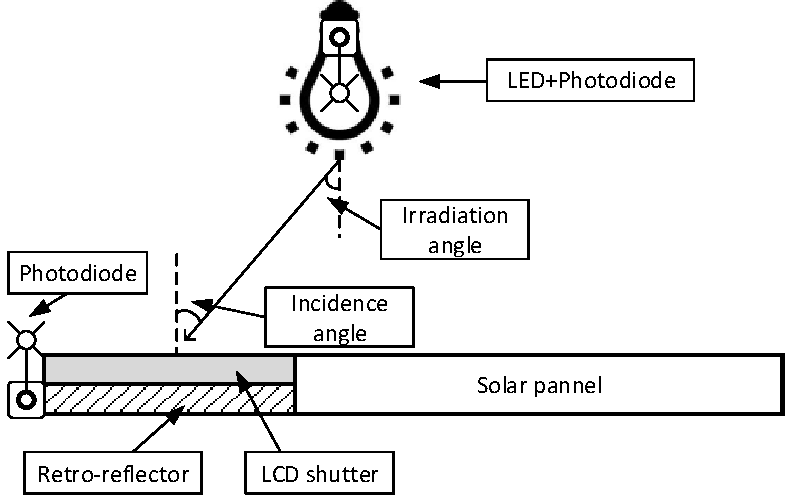
\includegraphics[width=.9\columnwidth]{system.pdf}
   \caption{System architecture.}
   \label{fig:system}
   \vskip -3mm
\end{figure}



Inspired by recent work on backscatter communication systems~\cite{abc1,abc4}, 
in this paper, we present the design and implementation of \textit{\retro} -- \textit{a low-power duplex VLC system} that consists of a reader (\reader) residing in the lighting infrastructure and tags ({\vitag}s) integrated in mobile devices or sensor nodes. The \reader is made up of an externally powered lighting LED, a light sensor (\eg photodiode) and the control circuits. The \vitag consists of a light sensor, a retro-reflective fabric, a transparent LCD shutter and the control circuits. One example tag implementation is shown in \figref{fig:system}. 

Central to \retro is the adoption of retro-reflective fabric which retrospectively reflects light, \ie bounces light back to the lighting source \textit{exactly along its incoming direction}. Its reflecting nature helps to establish an uplink over the \textit{same} visible light channel established by the high power lighting LED, which thus avoids using another high-power LED on the weak end and makes it possible to achieve the low-power design goal. %Rather, it resorts to backscattering the incoming light and communicates with the \reader over the same visible light channel. 
Its retrospective nature further not only allows arbitrary relative positioning between the lighting source and the tag, but also helps to concentrate the reflected light from a scattering light source. The two favorable properties render \retro an effective visible light based backscattering communication system. 

\retro works as follows. For the downlink (LED-to-tag), the LED in \reader switches on and off at a high frequency (\eg 1MHz, to avoid human perceptible flickering), turning the illuminating light into a communication carrier. Information bits are carried using certain modulation method (\eg Manchester coding). The light signals are picked up by the light sensor on \vitag and decoded to restore the information. 
For the uplink (tag-to-LED) communication, the same carrier is leveraged via reflection. To carry bits over the reflected light carrier, we cover the retro-reflector fabric with a transparent LCD that serves as a shutter, and adopt On-Off-Keying (OOK) modulation over the reflected light carrier by controlling the passing or blocking state of the LCD shutter.
%We further modulate the reflected light by applying an LCD as a modulator. By tuning the translucence of the LCD, we control the passing of the light reflected by the retro-reflector, and encode information bits using On-Off-Keying (OOK). 
The modulated reflected light carrier is then picked up by a photodiode on the \reader and decoded by a dedicated subsystem. 

Two major challenges arose in the design of the \retro system, especially the uplink. The root causes are the practicality considerations of the system and the low-power requirement of the tag. Specifically, the first challenge is the extremely weak and noisy signal (reflected by the remote tag) received by at the \reader. 
%When the communication range is large, the reflected light is very weak. 
We use a photodiode with wide field of view (FoV) on the \reader to avoid constraining the range of possible tag deployment. The wide FoV of the photodiode not only makes it less sensitive to the reflected lights (as only a tiny portion of its view actually corresponds to the retro-reflecting area of a tag), but also invites severe interference from the leakage and ambient reflection of the strong downlink signal and carrier.  
%The excitation of the photodiode caused by the reflected light is doomed to be small. Worse even, the wide FoV of the photodiode 
%\fyi{At the reader, the converted electrical signal is also interfered by the radio signals (\eg FM radio around 1MHz) and harmonics of the AC current. In addition, there is no clock synchronization between a \reader\ and \vitag(s).} 
Secondly, the low power consumption requirement of \vitag (in hope to achieve battery-free operation by only harvesting energy from the illuminating LED) entails careful design as well. The receiving (demodulation and decoding) unit and modulation unit (the LCD) on the \vitag consume significant energy. The LCD shutter leverages the electric field to control the arrangement of liquid crystal molecules (to polarize the light). It itself is a capacitor. Frequent charging and discharging the LCD consumes relatively significant energy, especially when the refresh rate is high. In addition, for sake of cost and energy consumption, we do not use any high precision oscillator on the \vitag. There is no clock synchronization between a \reader and \vitag(s) either.

\iffalse
\begin{figure}[tb!]
\centering
\minipage{.7\columnwidth}
      \subfigure[Front]{
        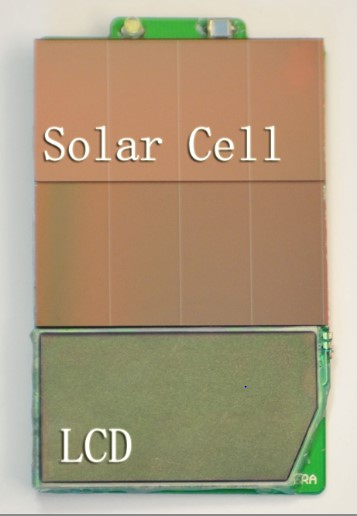
\includegraphics[width=0.45\columnwidth]{tag-front.jpg}
      } 
%      \hskip 1em
      \subfigure[Back]{
        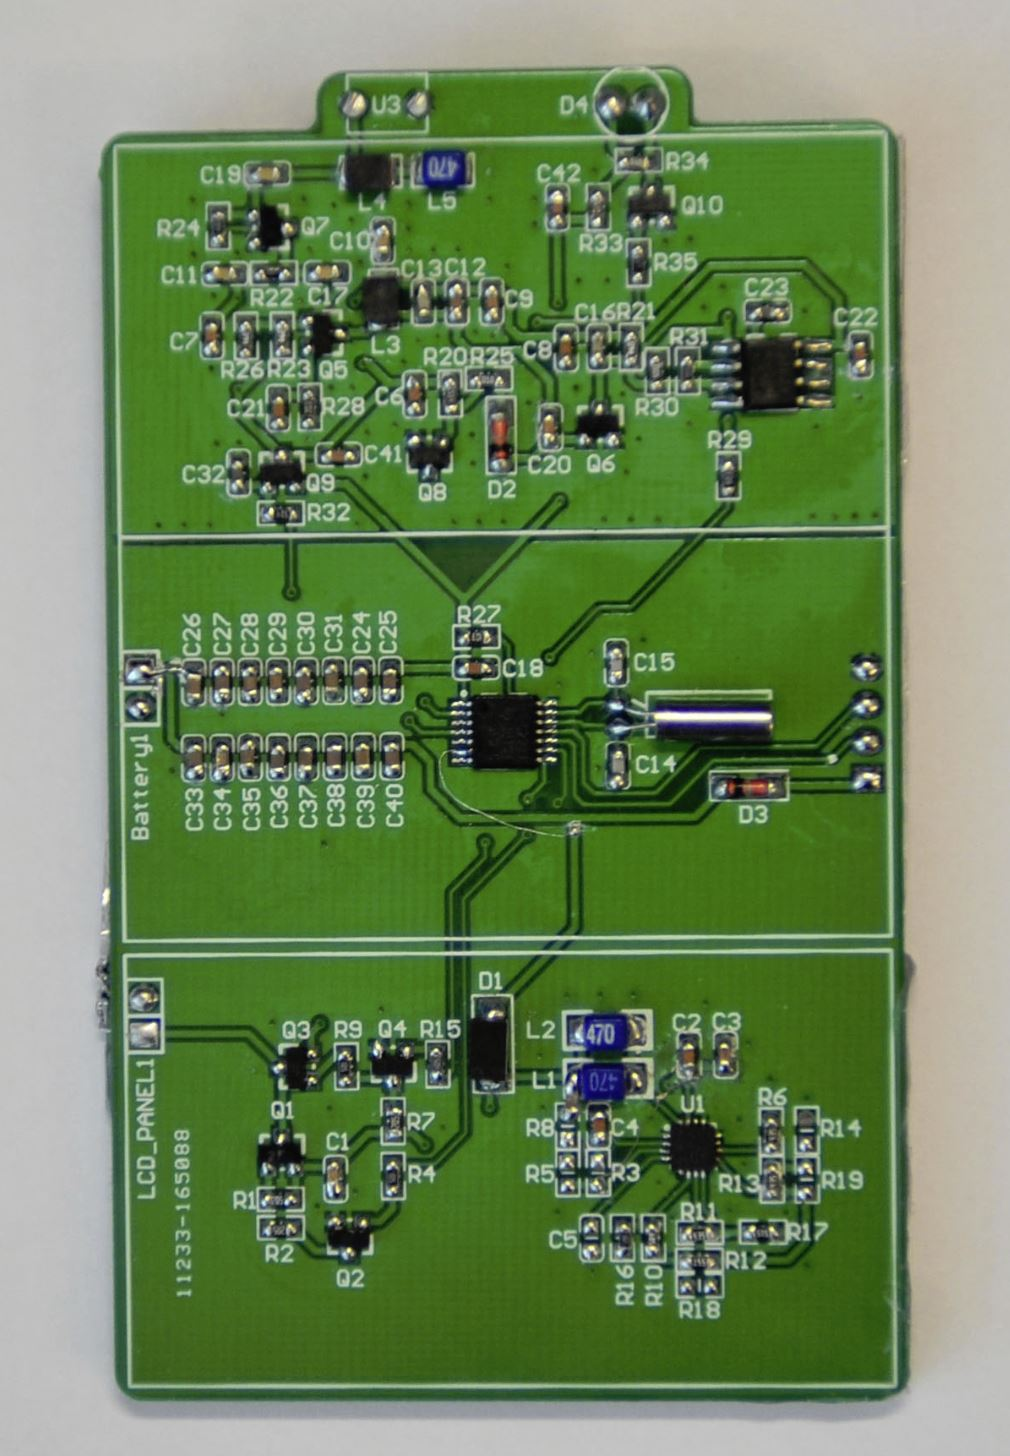
\includegraphics[width=0.45\columnwidth]{tag-back2.jpg}
      } 
\vspace{-1ex}      
\endminipage
\caption{\vitag prototype.}
\label{fig:proto}
%\vspace{-1em}      
\end{figure}
\fi

% \begin{Itemize}
% \item Handling the high throughput LED-transmitted data is power consuming. 
% \item Transmitting with the LCD at a high toggling frequency consumes even more power than the receiver.
% \item The LED receiver must handle clock offsets from the mobile end with low clock oscillating frequency.
% \item The LED receiver has to detect retro-reflected signals 3 orders of magnitude weaker than interfering LED transmissions.  
% \end{Itemize}

%\note{liqul: put using BLE for upper-link communication into discussion.}

We have addressed these challenges with the following design. We employ a differential amplifier in the \reader receiver to filter out the noises; we adopt a multi-stage amplification design with feedbacks for automatic gain control to pull the system away from self-excitation. With these designs, we amplify the signal by up to $120dB$ while ensuring the stability of the system. We devise a sliding-window multi-symbol match filter to handle possible clock offsets and drifts between the \reader and the \vitag. To achieve low power consumption of the \vitag, we have followed the principles of using as much analog components as possible, making the circuit work at the most energy-efficient (\ie close to cut-off) state, and seeking maximal energy reuse. In particular, we avoid energy-demanding analog-to-digital converters (ADCs) with a specially designed comparator. The microcontroller (MCU) in \vitag\ handles only simple tasks such as parity check and duty cycling, and the control of LCD states. We further design an energy reuse module that collects almost half of the LCD's discharging current.

%\textbf{\retro.} To understand our \vitag\ design on battery-free ID card-sized tags, consider an LCD whose emitted light can be manipulated by an additional small circuit inside the light bulb. This circuit embeds information in the light and modulates it, while keeping the brightness of the light the same without any flickering. On the \vitag\ side, a light sensor captures the light signal that conveys information from the LED. To conserve energy, \vitag\ only uses analog components to demodulate the signal without an ADC. Upon detecting data, a low-power micro-controller on \vitag\ is waked up for uplink data transmission. It drives up the LCD to flicker, therefore sending data back to the LED by backscattering the light with a retro-reflector behind the LCD. This uplink data can be captured by a light sensor placed on the LED, along with interferences caused by downlink transmission, nearby human and object movements, household electricity fluctuations, and so on. A specifically designed receiver associated with the LED then performs the time recovery and demodulates the signal. To get a network of \vitag\/s and LEDs into play, we design a Media Access Control (MAC) protocol to mediate the communications in LEDs' illumination range. 



\fyi{We have implemented several prototypes that demonstrate the effectiveness of our \retro design. We built battery-free \vitag device, which operates by harvesting  energy from the incoming light. \figref{fig:system} depicts the architecture of a \vitag. It is the same size of a credit card, one-third of the area being the retro-reflector and two-thirds the polycrystalline silicon solar cell. We made two types of \reader, modified from a normal LED bulb and a flashlight, respectively.} 
%We also explored the tradeoff between the solar panel area and the retro-reflector area for achieving a maximum working range in the worst case where the LED is the only light source, \ie no ambient light. 

%We demonstrated the design with a battery-free credit-card-sized \textbf{\vitag}, as shown in Fig.~\ref{fig:tag}, that harvests energy of off-the-shelf LED lights. We also explored the tradeoff between the solar panel area and the retro-reflector area for achieving a maximum working range at a typical $lux$ level. 

We evaluate our system in locations where illuminating LEDs are typically deployed such as office environments. We also evaluate in dark chambers for benchmark purpose. We measure the maximum communication range between the LED and the \vitag\ with various LED illumination levels, \vitag\ orientations, solar panel areas and retro-reflector areas. Our experiments show that our $8.2cm\times 5.2cm$ \vitag\ prototype can achieve $10kbps$ downlink speed and $0.5kbps$ uplink speed over distances of up to $1.7m$ in dark chambers and $2.4m$ in offices, under a $200\mu W$ power budget. We also demonstrate its merit in security by evaluating the area around the \vitag in which uplink transmissions can be sniffed. %\fyi{Experiments show \vitag's uplink transmission cannot be detected outside of a spindle-shaped area with a $0.2m$ radius. (Jiangtao: I think we should delete this sentence)}

\paragraph{Contributions} 
We make the following contributions:
\begin{Itemize}
\item We propose a practical bi-directional VLC primitive that works for small battery-free devices using retro-reflectors and LCDs and ordinary white LEDs. The design is well suited for the communication between a mobile or sensor device and the illuminating infrastructure.
\item We address various challenges through energy-efficient analog circuit design and energy reuse components on the \vitag, and weak signal detection and unsynchronized decoding scheme on the \reader.
\item We build and evaluate real working prototypes,  confirm the effectiveness of our design and provide a sense of its practicality. %with introduction of several real application scenarios. 
\end{Itemize}
%\begin{Itemize}
%\item We present \vitag, the first visible light duplex communication system design that operates on battery-free devices while retaining a small size for them.
%\item We develop a secure communication primitive applicable to RFID systems that acts against side sniffers and malicious transmitters.
%\item Finally, we present designs and build a prototype which shows how all of the above, from \vitag, modified LEDs, through to the network stack, can be implemented on credit-card sized battery-free devices at a low cost.
%\end{Itemize}


